%!TEX program = xelatex

\documentclass[12pt]{article}
\usepackage[UTF8]{ctex}
\usepackage{indentfirst}
\usepackage{lmodern}
\usepackage{setspace}
\usepackage{verbatim}
\usepackage{amsmath}
\usepackage{amsthm}
\usepackage{amssymb}
\usepackage{graphicx}
\usepackage{subfigure}
\usepackage{booktabs}
\usepackage{tabularx}
\usepackage{multirow}
\usepackage{multicol}
\usepackage{listings}
\usepackage{relsize}
\usepackage[usenames]{color}
\usepackage{fontspec}
\usepackage{geometry}
\geometry{left=2.0cm,right=2.0cm,top=2.5cm,bottom=2.5cm}

\usepackage{enumitem}
\setlist[enumerate]{listparindent=\parindent}

\usepackage[table]{xcolor}
\usepackage{array}
\usepackage[rightcaption]{sidecap}
\usepackage{hyperref}
\usepackage{float}
\hypersetup{
	colorlinks=true,
	linkcolor=black
}

\lstset{
	columns=fixed,
	numbers=left,
	numberstyle=\tiny\color{gray},
	frame=none,
	backgroundcolor=\color[RGB]{245,245,244},
	keywordstyle=\color[RGB]{40,40,255},
	numberstyle=\footnotesize\color{darkgray},
	commentstyle=\it\color[RGB]{0,128,0},
	stringstyle=\rmfamily\slshape\color[RGB]{128,0,0},
	showstringspaces=false,
	breaklines=true,
	language=python,
}

\newcommand{\myd}{\;\mathrm{d}}

\renewcommand{\arraystretch}{1.5}
\renewcommand\refname{参考网站}

\setlength{\parindent}{2em}
\addtolength{\parskip}{3pt}
\onehalfspacing
\graphicspath{{./figures/}{../assets/charts/}{../assets/}}

\usepackage{algorithm2e}
\usepackage{amssymb}

\newcommand{\daima}[1]{{\ttfamily{#1}}}

\setlist[enumerate]{itemsep=-4pt}
\setlist[itemize]{itemsep=-4pt}

\newcolumntype{H}{>{\centering\arraybackslash}p{2cm}}
\newcolumntype{C}{>{\centering\arraybackslash}p{2.4cm}}

\begin{document}
	\begin{titlepage}
		\vspace*{-2.5cm}
		\begin{figure}[h]
			\centering
			
\includegraphics[width=0.8\linewidth]{zjdx}
		\end{figure}
		\begin{figure}[h]
			\centering
			
\includegraphics[width=0.3\linewidth]{qsy}
		\end{figure}
		\vspace{-0.2cm}
		\begin{center}
			\Huge{\textbf{基于Q-Learning的Flappy Bird\\强化学习智能体设计}}\\
		\end{center}
		\vspace*{0.8cm}
		\begin{center}
			\larger[2]{
				\begin{tabular}{cc}
					姓\hspace{12pt}名 & \underline{\makebox[220pt]{黄鹤翔}}\\
					学\hspace{12pt}号 & \underline{\makebox[220pt]{3230106231}}\\
					院\hspace{12pt}系 & \underline{\makebox[220pt]{\kaishu 信息与电子工程学院}}\\
					指导老师 & \underline{\makebox[220pt]{\kaishu 金日成}}\\
				\end{tabular}
			}
		\end{center}
	\end{titlepage}

	\pagenumbering{arabic}

\newpage
\tableofcontents
\newpage

\section{引言}

Flappy Bird 是一款经典的 2D 横版躲避游戏，玩家需要操控小鸟通过上下间隙各异的管道障碍。由于游戏具有实时性、随机管道分布和重力影响，传统的手动控制或基于规则的方法难以泛化；而强化学习通过与环境交互来自动学习最优策略，非常适合此类序贯决策问题。

本报告基于 Q-Learning 算法为 Flappy Bird 训练智能体，完成了以下工作：
\begin{itemize}
	\item 补全 GameAI 类的 Q-Learning 代码框架，包括 Q 值查询、更新、动作选择等核心逻辑；
	\item 设计并比较了三种状态表示方法（作业示例、增强状态、扩展状态），并完成 bonus1 的状态设计实验；
	\item 通过网格搜索对学习率 $\alpha$、折扣因子 $\gamma$、探索率 $\varepsilon$、离散系数等参数进行系统性调整和性能比较；
	\item 设计奖励塑形方案（bonus2），在死亡惩罚基础上增加飞行姿态相关的密集反馈，并与原始奖励方案进行对比。
\end{itemize}

最终基础最佳模型保存在 \texttt{q\_base\_best.pkl} 中，50 局无步数限制评估的平均得分为 $\mathbf{165.18}$，最高分为 $\mathbf{984}$。在 bonus 实验中：bonus1 改良状态（\texttt{enhanced\_top}）将均分提升至 $\mathbf{275.40}$；bonus2 改良奖励（\texttt{shaped\_v2}）将均分提升至 $\mathbf{311.16}$；两者结合的组合模型均分达到 $\mathbf{571.50}$，最高分 $\mathbf{2620}$，保存在 \texttt{q\_combined\_best.pkl}/\texttt{q\_best.pkl} 中。所有数值均以无步数上限评估为准。
\begin{center}
	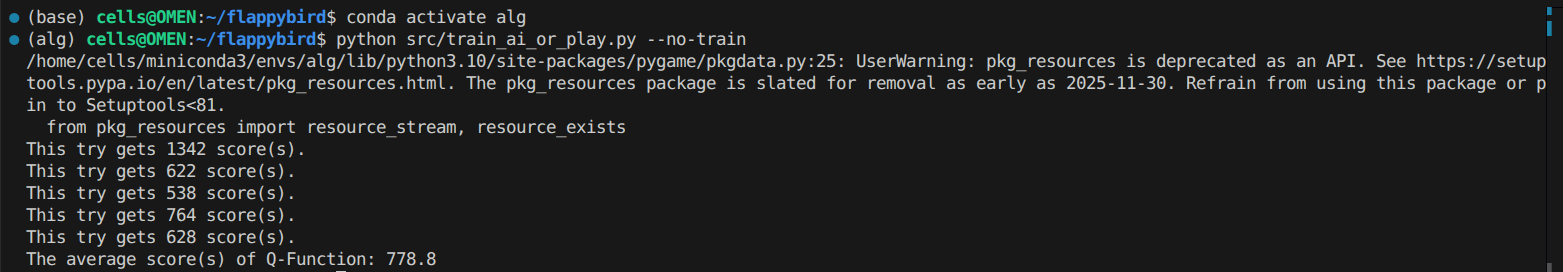
\includegraphics[width=0.9\textwidth]{res.png}
\end{center}
% \section{项目内容与代码结构}

% 本项目使用 Python 和 \texttt{flappy-bird-gymnasium} 游戏环境，基于表格型 Q-Learning 进行训练，不涉及神经网络或 DQN。项目核心代码文件说明如下：

% \begin{table}[H]
% 	\centering
% 	\begin{tabular}{ll}
% 		\toprule
% 		文件 & 功能说明 \\
% 		\midrule
% 		\texttt{src/q\_learning.py} & Q-Learning 智能体、状态处理、奖励塑形、训练/评估循环 \\
% 		\texttt{src/experiment.py} & 参数网格搜索、多线程训练、结果记录与模型保存 \\
% 		\texttt{src/watch\_best.py} & 加载最佳模型进行可视化或分数评估 \\
% 		\texttt{q\_best.pkl} & 最终基础最佳 Q 表模型（enhanced + death\_penalty, 100k） \\
% 		\texttt{q\_bonus1\_best.pkl} & bonus1 改良状态最佳模型（enhanced\_top + death\_penalty, 100k） \\
% 		\texttt{q\_bonus\_best.pkl} & bonus2 改良奖励最佳模型（enhanced + shaped\_v2, 100k） \\
% 		\texttt{q\_combined\_best.pkl} & 组合最佳模型（enhanced\_top + shaped\_v2, 100k） \\
% 		\texttt{scripts/eval\_unbounded.py} & 无步数限制评估脚本 \\
% 		\texttt{results/experiment\_results.csv} & 基础参数实验（18 组初筛 + 3 组复训）完整数据 \\
% 		\texttt{results\_bonus/experiment\_results.csv} & bonus 状态/奖励实验（8 组初筛 + 3 组复训）完整数据 \\
% 		\bottomrule
% 	\end{tabular}
% \end{table}

\section{算法原理}

\subsection{强化学习与马尔科夫决策过程}

Flappy Bird 游戏可以自然地建模为马尔科夫决策过程（Markov Decision Process, MDP），其核心五元组 $(S, A, P, R, \gamma)$ 与游戏元素的对应关系如下：

\begin{table}[H]
	\centering
	\begin{tabular}{cc}
		\toprule
		MDP 元素 & 本项目中对应的含义 \\
		\midrule
		状态 $s \in S$ & 小鸟和最近管道的相对位置、小鸟速度等离散化观测值 \\
		动作 $a \in A$ & $0$ 表示不扇动翅膀，$1$ 表示扇动（flap） \\
		奖励 $r = R(s, a, s')$ & 存活、通过管道、死亡、触顶等环境反馈 \\
		策略 $\pi(s)$ & 给定状态下选择最大 Q 值的动作 \\
		目标 & 最大化长期累积奖励，即尽量存活、通过更多管道 \\
		\bottomrule
	\end{tabular}
\end{table}

强化学习的核心思想是：智能体在环境中不断试错，收集 $(s_t, a_t, r_{t+1}, s_{t+1})$ 四元组样本，通过学习使长期累积奖励最大化。在游戏早期，智能体几乎不知道何时该扇动，因此会频繁撞管或坠地；随着训练进行，智能体逐渐将"哪些动作导致更高长期回报"记录在 Q 表中。测试时，只需查询当前状态下两个动作的 Q 值，选择 Q 值更大的动作即可。

\subsection{Q-Learning 算法}

Q-Learning 是一种无模型的基于样本的 Q 值迭代方法（off-policy 的时序差分学习）。它直接从环境交互中采样，逐步逼近最优动作价值函数 $Q^*(s, a)$，其核心更新公式为：

\begin{equation}
	Q(s, a) \leftarrow Q(s, a) + \alpha \left[ r + \gamma \max_{a'} Q(s', a') - Q(s, a) \right]
	\label{eq:q_learning}
\end{equation}

其中各符号的含义如下：

\begin{itemize}
	\item $s$：当前状态（old\_state）；
	\item $a$：当前采取的动作（action）；
	\item $r$：执行动作后立即获得的奖励（reward）；
	\item $s'$：执行动作后转移到的新状态（new\_state）；
	\item $\alpha$：学习率（Learning Rate），$\alpha \in [0, 1]$，决定新样本对旧 Q 值的覆盖速度。$\alpha$ 越接近 1，旧值被覆盖得越快；$\alpha$ 越接近 0，学习越保守；
	\item $\gamma$：折扣因子（Discount Factor），$\gamma \in [0, 1]$，决定智能体对即时奖励和长远未来奖励的重视程度。$\gamma$ 越接近 1，越重视长远收益；$\gamma$ 越接近 0，越短视；
	\item $\max_{a'} Q(s', a')$：对从新状态 $s'$ 出发所能获得的未来最优回报的估计。
\end{itemize}

公式 \eqref{eq:q_learning} 中，方括号内的 $[r + \gamma \max_{a'} Q(s', a')]$ 构成对 $Q(s, a)$ 的新估计（称为 TD target），而 $(Q_{\text{target}} - Q_{\text{old}})$ 是时序差分误差（TD Error）。整个更新过程体现了 Q-Learning "用新样本纠正旧估计"的迭代优化思想。

\subsection{$\varepsilon$-greedy 探索策略}

Q-Learning 的训练需要兼顾探索（Exploration）和利用（Exploitation）。本系统采用 $\varepsilon$-greedy 策略：

\begin{equation}
	a = \begin{cases}
		\text{随机选择合法动作}, & \text{以概率 } \varepsilon \\
		\arg\max_a Q(s, a),   & \text{以概率 } 1 - \varepsilon
	\end{cases}
	\label{eq:epsilon_greedy}
\end{equation}

若多个动作具有相同的最大 Q 值（例如两个动作 Q 值均为 0），则在并列最优动作中随机选择一个。这一设计在训练早期尤为重要：当 Q 表中大量条目尚未被访问时，并列最优动作的随机选择提供了天然的探索能力。

\section{算法实现}

本节阐述 GameAI 类的核心实现，并结合公式 \eqref{eq:q_learning} 的数学原理对关键代码进行注释说明。

\subsection{数据存储与 Q 值查询}

Q 表使用 Python 字典存储映射关系 \texttt{(tuple(state), action)} $\to$ \texttt{q\_value}。未出现在字典中的状态—动作对默认返回 0，这体现了 Q-Learning 的"零初始化"原则：

\begin{lstlisting}[language=Python, caption={GameAI 初始化与 Q 值查询}, label={lst:init}]
class GameAI():
    def __init__(self, alpha=0.5, gamma=1, epsilon=0.1, rng=None):
        """
        初始化智能体：
        * self.q: 一个字典，表示 Q-Function
          从 (状态, 动作) 元组 映射到 Q 值
          未出现在字典中的条目 Q 值默认为 0
        * alpha: 学习率，控制新样本对旧估值的覆盖速度
        * gamma: 折扣因子，决定对未来奖励的重视程度
        * epsilon: 探索概率，用于 epsilon-greedy 策略
        """
        self.q = dict()
        self.alpha = alpha
        self.gamma = gamma
        self.epsilon = epsilon
        self.rng = rng or random

    def get_q_value(self, state: List[int], action: int) -> float:
        """
        查询 (state, action) 对的 Q 值
        若该条目不存在则返回 0——即 Q 表的零初始化原则
        """
        return self.q.get((tuple(state), action), 0)

    def best_future_reward(self, state: List[int]) -> float:
        """
        给定状态 state，计算 max_{a'} Q(state, a')
        这是公式 (1) 中的核心子项
        """
        actions = self.available_actions(state)
        if not actions:
            return 0
        return max(self.get_q_value(state, action) for action in actions)
\end{lstlisting}

\subsection{Q 值更新}

\texttt{update} 方法直接实现公式 \eqref{eq:q_learning}：

\begin{lstlisting}[language=Python, caption={Q-Learning 更新}, label={lst:update}]
    def update(self, old_state, action, new_state, reward):
        """
        基于一个 (s, a, s', r) 样本，按照 Q-Learning 公式更新 Q 值

        公式: Q(s, a) <- Q(s, a) + alpha * [r + gamma * max_{a'} Q(s', a') - Q(s, a)]
        亦即: Q_new = Q_old + alpha * (TD_target - Q_old)
        """
        old_q = self.get_q_value(old_state, action)
        # 计算 max_{a'} Q(s', a') — 对未来最优回报的估计
        future_reward = self.best_future_reward(new_state)
        # TD target: r + gamma * max_{a'} Q(s', a')
        new_estimate = reward + self.gamma * future_reward
        # Q-learning 更新公式
        self.q[(tuple(old_state), action)] = old_q + self.alpha * (new_estimate - old_q)
\end{lstlisting}

\subsection{动作选择}

\texttt{choose\_action} 方法实现公式 \eqref{eq:epsilon_greedy} 的 $\varepsilon$-greedy 策略：

\begin{lstlisting}[language=Python, caption={动作选择}, label={lst:action}]
    def choose_action(self, state, use_epsilon=True):
        """
        给定状态 state，返回要采取的动作:
        - 若 use_epsilon 为 True 且随机数 < epsilon，随机探索
        - 否则选择当前 Q 值最大的动作（利用已知知识）
        - 若多个动作 Q 值相同，在并列最优中随机选择
        """
        actions = sorted(self.available_actions(state))
        # epsilon 概率随机探索
        if use_epsilon and self.rng.random() < self.epsilon:
            return self.rng.choice(actions)
        # 找出具有最大 Q 值的所有动作
        best_value = max(self.get_q_value(state, action) for action in actions)
        best_actions = [
            action for action in actions
            if self.get_q_value(state, action) == best_value
        ]
        # 在并列最优动作中随机选择
        return self.rng.choice(best_actions)

    @classmethod
    def available_actions(cls, state):
        """
        返回该状态下的所有合法动作
        Flappy Bird 中为 {0, 1}: 0 = 不扇动, 1 = 扇动翅膀
        """
        actions = set()
        actions.add(0)
        actions.add(1)
        return actions
\end{lstlisting}

\subsection{训练循环}

训练循环是 Q-Learning 算法步骤 2-4（采样 → 更新 → 重复）的具体实现：

\begin{lstlisting}[language=Python, caption={训练循环}, label={lst:train}]
def train(iteration, alpha, gamma, epsilon, obs_mul_factor=30,
          seed=42, death_penalty=-1000, state_mode="enhanced",
          reward_mode="death_penalty"):
    """
    通过让 AI 进行 iteration 次游戏来进行 Q-Learning 训练
    每次游戏从重置环境开始，直到小鸟死亡或步数超限
    """
    rng = random.Random(seed)
    player = GameAI(alpha=alpha, gamma=gamma, epsilon=epsilon, rng=rng)
    env = gymnasium.make("FlappyBird-v0", render_mode=None, use_lidar=False)

    # 进行多次游戏，每次为一条完整的 episode
    for i in range(iteration):
        obs, _ = env.reset()
        while True:
            # 第一步：将观测值转化为离散状态
            state = process_obs(obs, obs_mul_factor, state_mode)
            # 第二步：使用 epsilon-greedy 选择动作
            action = player.choose_action(state)
            # 第三步：执行动作，获取 next_obs, reward, terminated
            next_obs, reward, terminated, _, info = env.step(action)
            # 第四步：应用奖励塑形，将死亡惩罚放大为 -1000
            reward = shape_reward(next_obs, reward, terminated, action,
                                  reward_mode=reward_mode,
                                  death_penalty=death_penalty)
            # 第五步：Q-Learning 更新 Q 表
            player.update(state, action,
                          process_obs(next_obs, obs_mul_factor, state_mode),
                          reward)
            if terminated:
                break
            obs = next_obs
    env.close()
    return player
\end{lstlisting}

\section{实验}

\subsection{基础参数实验}

\subsubsection{实验设置}

实验采用两阶段策略：初筛阶段用较少训练局数（30000 局）快速扫描参数空间，选出最优的 $3$ 组候选；复训阶段将这些候选用更多局数（100000 局）精细训练并全面评估。

基础实验初筛共 $18$ 组参数组合，覆盖以下范围：

\begin{itemize}
	\item 学习率 $\alpha \in \{0.5, 0.6, 0.7, 0.8\}$
	\item 折扣因子 $\gamma \in \{0.90, 0.95, 0.99\}$
	\item 探索率 $\varepsilon \in \{0.0, 0.05, 0.10\}$
	\item 状态离散系数 $obs\_mul\_factor \in \{24, 30, 36\}$
\end{itemize}

每组初筛训练 $30000$ 局、评估 $20$ 局；前 $3$ 组复训 $100000$ 局、评估 $50$ 局。训练每局最多 $1000$ 步，防止单个训练回合过长。评估阶段最初设置了 $5000$ 步上限，但经分析发现此上限会截断高分游戏（大量游戏在达到步数上限时被强制终止，导致最高分被错误地记录为 $132$），因此本报告中所有复训评估数据均以取消步数上限后的重新评估结果为准。

\subsubsection{初筛结果}

\begin{figure}[H]
	\centering
	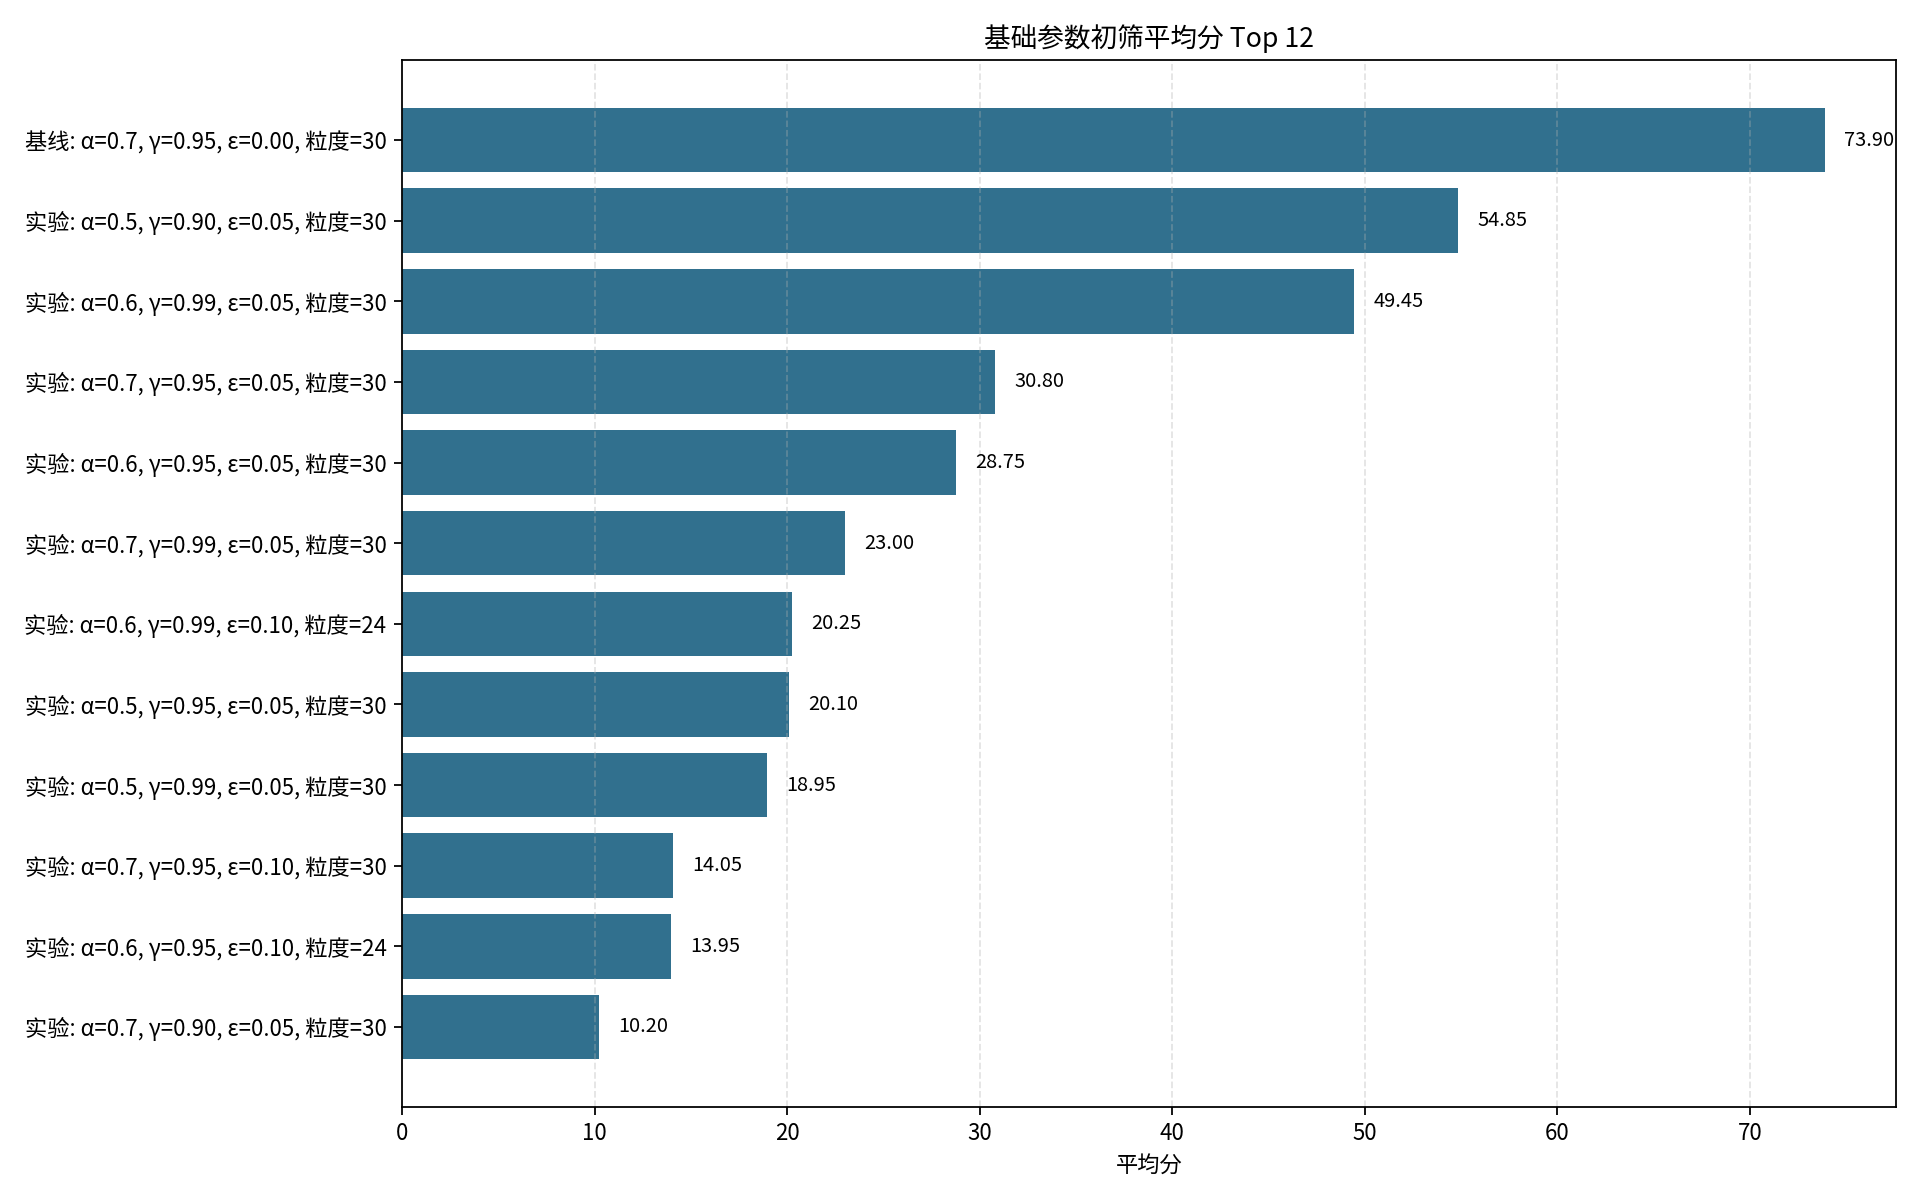
\includegraphics[width=0.9\textwidth]{base_screen_top12.png}
	\caption{基础参数初筛 Top 12 平均分}
	\label{fig:screen}
\end{figure}

如图 \ref{fig:screen} 所示，初筛前三名为：

\begin{table}[H]
	\centering
	\caption{初筛前三参数组合}
	\label{tab:screen_top3}
	\begin{tabular}{cccccc}
		\toprule
		参数组 & $\alpha$ & $\gamma$ & $\varepsilon$ & $obs\_mul\_factor$ & 初筛均分 \\
		\midrule
		基线参数 & $0.7$ & $0.95$ & $0.00$ & $30$ & $73.90$ \\
		低速学习·快折扣·小探索 & $0.5$ & $0.90$ & $0.05$ & $30$ & $54.85$ \\
		中速学习·慢折扣·小探索 & $0.6$ & $0.99$ & $0.05$ & $30$ & $49.45$ \\
		\bottomrule
	\end{tabular}
\end{table}

值得注意的是，初筛第一名（基线参数）的 $\varepsilon = 0$，即没有显式随机探索。这并不等于完全没有探索，原因如前所述：训练早期大量未访问的状态—动作对 Q 值均为 0，并列最优动作的随机选择机制已经引入了足够的随机性。额外 $\varepsilon$ 探索在 Flappy Bird 中尤其危险，因为随机扇动极易导致撞管或触顶——而死亡惩罚为 $-1000$，远超存活和过管奖励。

\subsubsection{复训结果}

\begin{figure}[H]
	\centering
	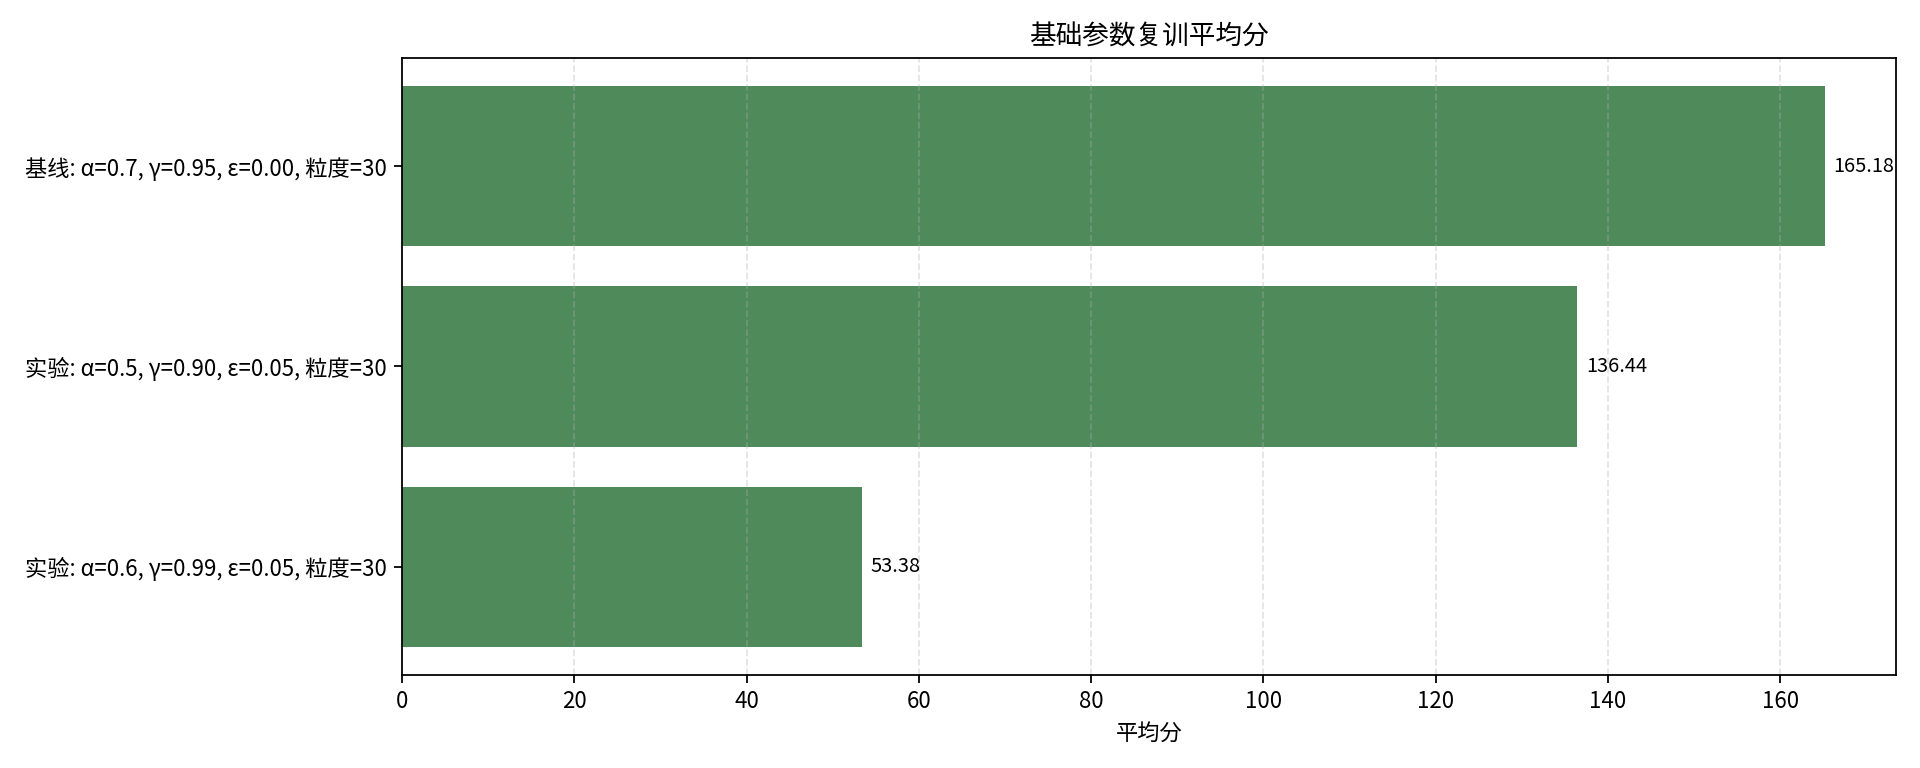
\includegraphics[width=0.85\textwidth]{base_retrain.png}
	\caption{基础参数复训结果}
	\label{fig:retrain}
\end{figure}

如图 \ref{fig:retrain} 和表 \ref{tab:retrain} 所示，复训后基线参数继续领先。

\begin{table}[H]
	\centering
	\caption{复训三组完整结果}
	\label{tab:retrain}
		\begin{tabular}{ccccccc}
		\toprule
		参数组 & $\alpha$ & $\gamma$ & $\varepsilon$ & 复训均分 & 最低分 & 最高分 \\
		\midrule
		基线参数 & $0.7$ & $0.95$ & $0.00$ & $\mathbf{165.18}$ & $3$ & $984$ \\
		低速·快折扣·小探索 & $0.5$ & $0.90$ & $0.05$ & $136.44$ & $2$ & $669$ \\
		中速·慢折扣·小探索 & $0.6$ & $0.99$ & $0.05$ & $53.38$ & $4$ & $250$ \\
		\bottomrule
		\end{tabular}
	\end{table}

最终基础最佳模型为"基线参数"组（$\alpha=0.7, \gamma=0.95, \varepsilon=0.0, obs\_mul\_factor=30$），保存为 \texttt{q\_best.pkl}。Q 表规模为 $14912$ 条，训练耗时约 $903.8$ 秒。

\subsubsection{最佳模型 50 局分数分布}

\begin{figure}[H]
	\centering
	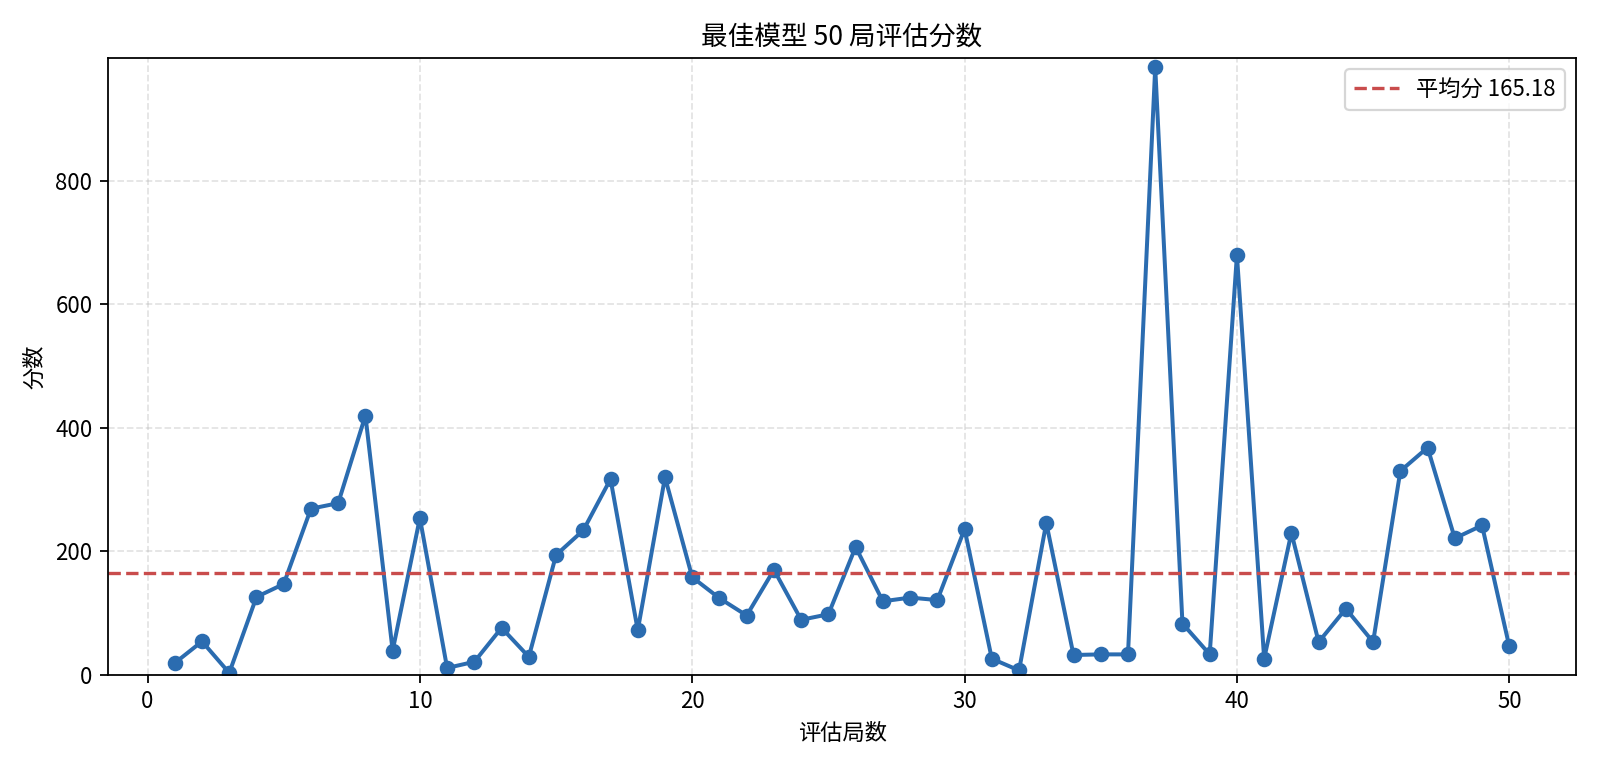
\includegraphics[width=0.85\textwidth]{best_scores_line.png}
	\caption{最佳模型 50 局评估分数走势}
	\label{fig:best_scores}
\end{figure}

如图 \ref{fig:best_scores} 所示，50 局评估分数存在较大波动（标准差 $175.66$），最低 $3$ 分，最高 $984$ 分。这是因为 Flappy Bird 中管道序列随机生成，且一次错误 flap 可能迅速导致死亡。高分游戏中，模型已经掌握了可靠的穿管策略，能够持续存活并通过大量管道；而低分游戏往往由于管道在关键位置出现时离散化状态恰好落入 Q 表未充分优化的区域。值得注意的是，旧的实验中由于设定了 5000 步的评估上限，绝大多数高分游戏被强制截断在 132 分左右（旧报告称 21/50 局达到 132 分，实则为步数截顶），取消步数上限后模型的真实最高分达到 984，平均分也从 90.52 提升至 165.18。

\subsubsection{参数影响分析}

下面结合实验数据，从理论角度分析各参数对模型性能的具体影响。

\begin{figure}[H]
	\centering
	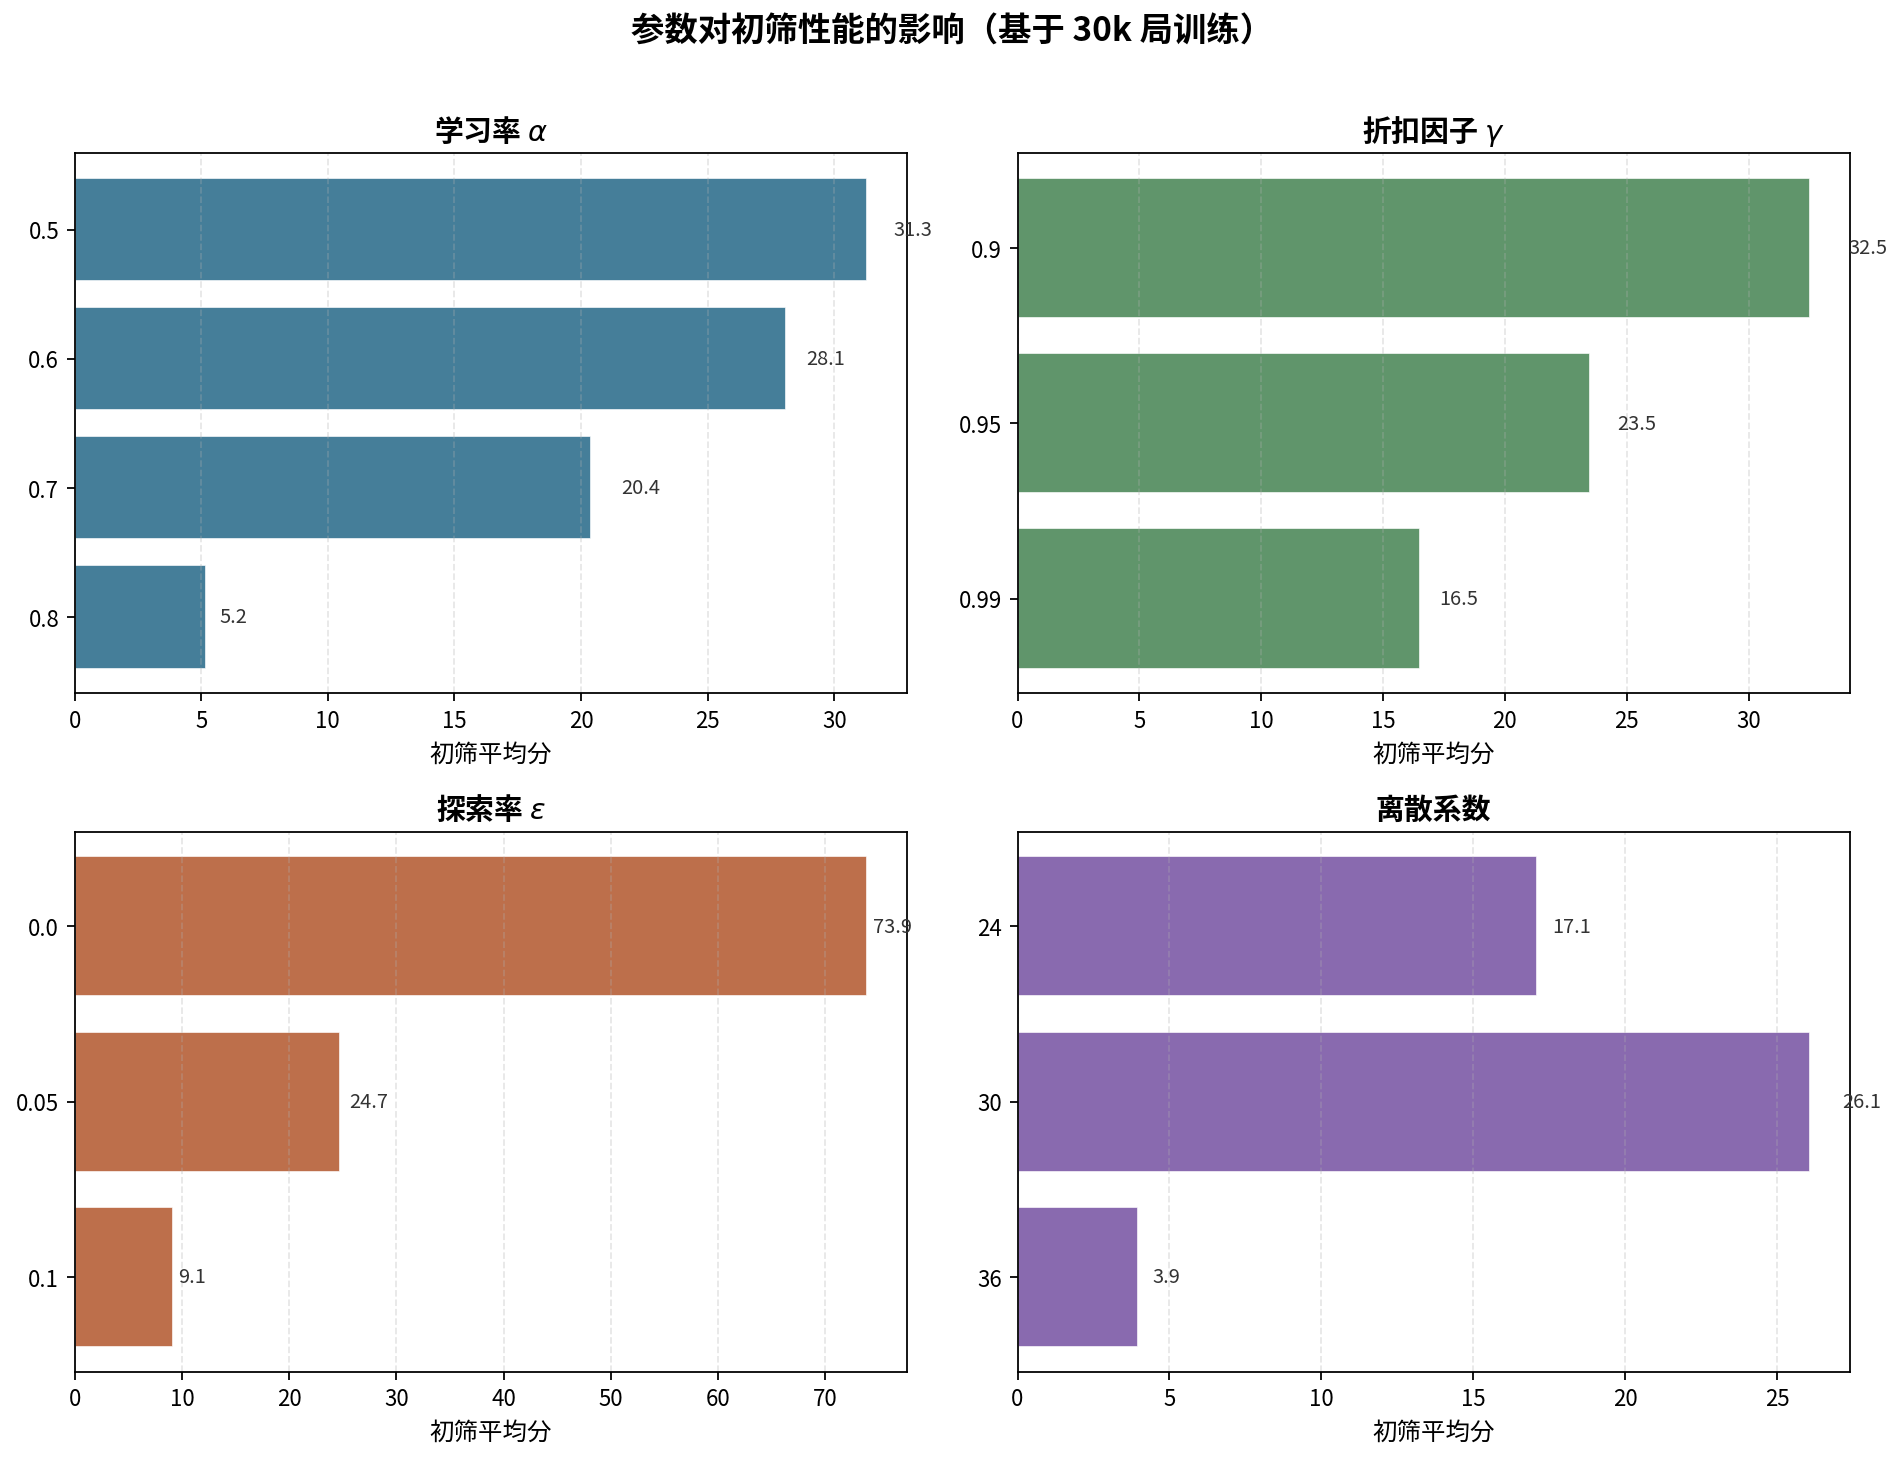
\includegraphics[width=0.95\textwidth]{param_analysis.png}
	\caption{各参数对初筛性能的影响（基于 18 组 30k 局训练，按参数值分组取平均）}
	\label{fig:param_analysis}
\end{figure}

如图 \ref{fig:param_analysis} 所示，随着各参数取值变化，初筛平均分呈现明显趋势。以下结合具体实验数据逐一分析。

\paragraph{学习率 $\alpha$}

\begin{itemize}
	\item $\alpha = 0.7$ 的基线参数表现最好（复训均分 $165.18$），$\alpha = 0.5$ 紧随其后（$136.44$）。这说明在该任务中，较大学习率有利于快速吸收新样本，尤其是在 100000 局的训练量下。
	\item $\alpha = 0.8$ 的配置在初筛仅为 $2.70$ 分（第 19 名），远低于同行其他参数，原因是过大的学习率使得 Q 值更新过于激进，导致对单次样本的噪声过度敏感，估值震荡剧烈。
	\item $\alpha = 0.6$ 结合低速探索（$\varepsilon = 0.05$）的配置在初筛表现较差，部分组合仅有 $28.75$ 分，可能是学习速度不足导致策略未充分收敛。
\end{itemize}

\paragraph{折扣因子 $\gamma$}

\begin{itemize}
	\item $\gamma = 0.95$ 在所有 top 配置中表现最好。它既不过于短视（$\gamma = 0.90$ 只关注前几步收益，难以形成长远过管策略），也不过于长视（$\gamma = 0.99$ 使得早期 death penalty 的回传衰减极慢，增加了优化难度）。
	\item 在 Flappy Bird 任务中，管道间隙大约每 $50$–$60$ 帧出现一次。$\gamma = 0.99$ 意味着 $50$ 步后的奖励仍有 $0.99^{50} \approx 0.605$ 的权重，可能导致智能体对过于遥远的事件信号产生不合理关联，降低训练稳定性。
	\item $\gamma = 0.90$ 则过于重视近期收益，$10$ 步后信号已衰减至 $0.90^{10} \approx 0.349$，不利于形成"穿越当前管道→为下一管道做准备"的远见性策略。
\end{itemize}

\paragraph{探索率 $\varepsilon$}

\begin{itemize}
	\item $\varepsilon = 0$ 在所有同参数对比中表现最好。核心原因是：Flappy Bird 中一次随机扇动容易导致撞管即死（$-1000$ 惩罚），而存活奖励（$+0.1$）、过管奖励（$+1.0$）远低于此，单次随机探索的期望代价极大。因此 $\varepsilon > 0$ 的显式探索在此估值量级下弊大于利。
	\item $\varepsilon = 0.05$ 的配置仍能找到可用策略（如 $a=0.5, g=0.90, \varepsilon=0.05$ 复训均分 $136.44$），但总体弱于基线。
	\item $\varepsilon = 0.10$ 的配置几乎全部表现最差，如 $a=0.7, g=0.99, \varepsilon=0.10$ 仅 $3.80$ 分（倒数第二），说明过强的随机探索严重干扰了 Q 表的收敛。
\end{itemize}

\paragraph{状态离散系数 \texttt{obs\_mul\_factor}}

\begin{itemize}
	\item $obs\_mul\_factor = 30$ 在所有对比中表现最好。它提供了合理的状态空间分辨率：既能区分不同的飞行位置，又不至于使 Q 表过于稀疏。
	\item $obs\_mul\_factor = 24$（较粗粒度）对应的初筛均分偏低（如 $a=0.6, g=0.99, \varepsilon=0.10$ 仅 $20.25$ 分），因为粗糙的离散化混淆了需要精细区分的状态，例如"接近上管道"和"接近下管道"可能被映射到同一个状态键。
	\item $obs\_mul\_factor = 36$（较细粒度）对应的组合几乎是全部最差（如 $a=0.7, g=0.99, \varepsilon=0.10$ 仅 $3.95$ 分），因为过于精细的离散化使得状态空间呈指数级膨胀，而 30000/100000 局的训练量无法充分覆盖每个状态—动作对，Q 表大量条目保持为 $0$ 的初始值。
\end{itemize}

\subsection{Bonus 状态与奖励实验}

\subsubsection{状态表示改良（bonus1）与实验结果}

\textbf{环境观测值 $obs$}

环境返回 12 维归一化观测向量，各维度的含义如表 \ref{tab:obs} 所示：

\begin{table}[H]
	\centering
	\caption{环境观测值 $obs$ 各维度含义}
	\label{tab:obs}
	\begin{tabular}{cc}
		\toprule
		下标 & 含义 \\
		\midrule
		$obs[0:3]$ & 第一个可见管道：水平位置、上管道底端、下管道顶端 \\
		$obs[3:6]$ & 第二个管道：水平位置、上管道底端、下管道顶端 \\
		$obs[6:9]$ & 第三个管道：水平位置、上管道底端、下管道顶端 \\
		$obs[9]$   & 小鸟纵向位置（归一化） \\
		$obs[10]$  & 小鸟纵向速度（归一化） \\
		$obs[11]$  & 小鸟旋转角（归一化） \\
		\bottomrule
	\end{tabular}
\end{table}

由于 Q 表需要可哈希的离散键值，所有连续观测值乘以 \texttt{obs\_mul\_factor}$=30$ 并取整。

\textbf{最近管道选择}

画面中可能同时存在多个管道，但控制当前动作最有意义的是"与小鸟最近且尚未完全通过的管道"。代码中通过比较管道水平位置 $x$ 与小鸟固定水平位置 $0.2$ 来决定：

\begin{itemize}
	\item 若第一个管道的最右端已完全位于小鸟身后（即 $obs[0] + pipe\_width < 0.2$），则使用第二组管道；
	\item 否则仍使用第一组管道。
\end{itemize}

这避免了小鸟已通过某管道后，状态仍被旧的障碍物信息干扰。

\textbf{状态表示方法设计}

本项目实现了三种 \texttt{state\_mode}，从简单到精细地逐步丰富状态向量，如表 \ref{tab:state_modes} 所示。

\begin{table}[H]
	\centering
	\caption{四种状态表示方法对比}
	\label{tab:state_modes}
	\small
	\begin{tabularx}{\textwidth}{cclX}
		\toprule
		\texttt{state\_mode} & 维 & 特征向量 & 设计思路 \\
		\midrule
		\texttt{example} & 3 &
		$\begin{bmatrix}
			pipe\_x - player\_x \\
			pipe\_bottom - player\_y \\
			player\_v
		\end{bmatrix}$ &
		作业示例。关注水平距离、下管道距离和小鸟速度。\\
		\midrule
		\texttt{enhanced} & 4 &
		$\begin{bmatrix}
			pipe\_x - player\_x \\
			player\_y - gap\_center \\
			pipe\_bottom - player\_y \\
			player\_v
		\end{bmatrix}$ &
		基础最佳。新增缺口中心垂直差，直接表达"飞向中心"目标。100k 均分 165.18。\\
		\midrule
		\texttt{enhanced\_top} & 5 &
		$\begin{bmatrix}
			pipe\_x - player\_x \\
			player\_y - gap\_center \\
			pipe\_bottom - player\_y \\
			player\_v \\
			player\_y - pipe\_top
		\end{bmatrix}$ &
		\textbf{bonus1 方案}。新增上管道距离，提供间隙大小和上边界信息。仅 +1 维，Q 表 $\sim$21k。100k 均分 $\mathbf{275.40}$（+67\%）。\\
		\midrule
		\texttt{bonus} & 6 &
		$\begin{bmatrix}
			pipe\_x - player\_x \\
			player\_y - gap\_center \\
			player\_y - pipe\_top \\
			pipe\_bottom - player\_y \\
			player\_v \\
			player\_rot
		\end{bmatrix}$ &
		含上管道距离和旋转角。6 维导致 Q 表稀疏（$\sim$26k），旋转角噪声大、信息增益低。100k 仅 67.74。\\
		\bottomrule
	\end{tabularx}
\end{table}


\textbf{性能比较}

图 \ref{fig:state_compare} 展示了在相同训练参数（$\alpha=0.7, \gamma=0.95, \varepsilon=0.0$、30000 局训练）下，四种方案的初筛平均得分对比。

\begin{figure}[H]
	\centering
	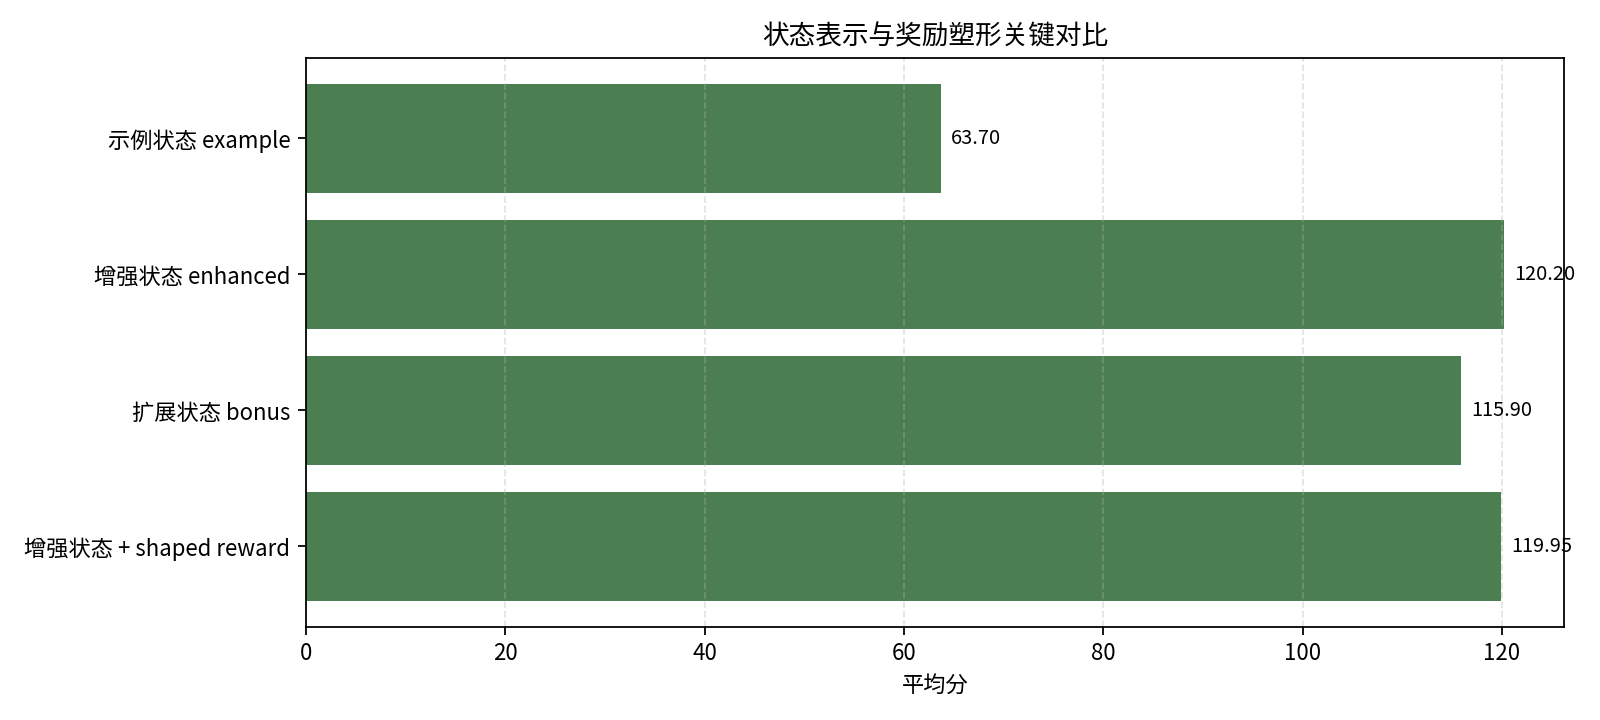
\includegraphics[width=0.85\textwidth]{state_reward_key_compare.png}
	\caption{状态表示与奖励塑形关键对比}
	\label{fig:state_compare}
\end{figure}

从图 \ref{fig:state_compare} 可以得出以下结论：

\begin{enumerate}
	\item 示例状态 \texttt{example}（平均分 $63.70$）的性能明显低于增强状态 \texttt{enhanced}（平均分 $120.20$）。核心原因在于 \texttt{example} 仅保留了"与下管道距离"，忽略了小鸟在整个管道间隙中的相对位置。\texttt{enhanced} 通过加入"到缺口中心的垂直差"，使状态能够区分小鸟在间隙上部和下部的不同情况。

	\item 扩展状态 \texttt{bonus}（6 维，含旋转角）在初筛中表现不错（$115.90$），但复训后降至 $67.74$，原因是旋转角增加信息增益有限但导致状态空间过度膨胀。

	\item \textbf{bonus1 最佳方案 \texttt{enhanced\_top}}（5 维）：在 \texttt{enhanced} 基础上仅增加 $player\_y - pipe\_top$（到上管道的垂直距离）。100k 局训练后均分达到 $\mathbf{275.40}$，相比 \texttt{enhanced} 的 $165.18$ 提升了 67\%。关键原因：该特征额外提供了间隙大小信息——当上下管道间距很窄时，小鸟需要更精准地控制高度，而知道上边界位置可以提前判断碰撞风险。同时仅增加 1 维，Q 表规模（$\sim$21k）仍然可控。
\end{enumerate}

结论：\texttt{enhanced\_top} 状态表示在表达能力和 Q 表规模之间取得了最佳平衡，被选作 bonus1 的最终方案（模型保存为 \texttt{q\_bonus1\_best.pkl}）。

\subsubsection{奖励塑形改良（bonus2）与实验结果}

\textbf{环境原始奖励与死亡惩罚}

环境为智能体提供离散奖励信号：

\begin{table}[H]
	\centering
	\caption{环境原始奖励}
	\label{tab:reward_env}
	\begin{tabular}{cc}
		\toprule
		事件 & 奖励值 \\
		\midrule
		每帧存活 & $+0.1$ \\
		成功通过管道 & $+1.0$ \\
		死亡 & $-1.0$ \\
		触顶 & $-0.5$ \\
		\bottomrule
	\end{tabular}
\end{table}

在本项目的基础奖励方案（\texttt{reward\_mode="death\_penalty"}）中，保留存活和过管奖励不变，但将死亡奖励从 $-1$ 放大为 $-1000$。原因在于：Flappy Bird 的核心目标首先是不死，只有活着才能持续获得分数。如果死亡惩罚与过管奖励（$+1.0$）差距不足以拉开，智能体可能无法充分重视危险状态，导致 Q 表难以收敛到安全稳定的策略。死亡惩罚的放大使得时序差分误差在每次死亡后迅速向后传播，将"导致死亡的动作"的 Q 值压至很低的水平。

\textbf{奖励塑形方案}

bonus2 实现了 \texttt{reward\_mode="shaped"}，在死亡惩罚之上增加飞行姿态相关的密集中间反馈（Reward Shaping）：

\begin{equation}
\begin{aligned}
	\text{shaped\_reward} =
	& \ \text{env\_reward} \quad \text{（环境基础奖励）} \\
	&+ \text{center\_bonus} \quad \text{（缺口中奖励）} \\
	&- \text{velocity\_penalty} \quad \text{（速度惩罚）} \\
	&- \text{flap\_penalty} \quad \text{（扇动惩罚）} \\
	&- \text{top\_penalty} \quad \text{（触顶惩罚）}
\end{aligned}
\label{eq:shaped}
\end{equation}

各项具体实现和设计目的如下：

\begin{lstlisting}[language=Python, caption={奖励塑形实现}, label={lst:shaped}]
def shape_reward(obs, reward, terminated, action,
                 reward_mode="death_penalty", death_penalty=-1000):
    if reward == -1:
        return death_penalty            # 将死亡奖励放大为 -1000
    if reward_mode == "death_penalty":
        return reward                   # 基础方案：只放大死亡惩罚

    # --- 以下是奖励塑形方案 ---
    pipe_start, _ = _nearest_pipe(obs)
    pipe_top = obs[pipe_start + 1]      # 最近管道的上管底端位置
    pipe_bottom = obs[pipe_start + 2]   # 最近管道的下管顶端位置
    player_y = obs[9]
    player_v = obs[10]
    gap_center = (pipe_top + pipe_bottom) / 2  # 管道间隙中心

    # 中心奖励：小鸟越接近管道间隙中心，奖励越高（最大 +0.2）
    # 当小鸟与中心距离大于 0.25 时奖励为 0
    center_bonus = max(0, 1 - abs(player_y - gap_center) * 4) * 0.2

    # 速度惩罚：垂直速度越大惩罚越大，鼓励平稳飞行，避免剧烈震荡
    velocity_penalty = abs(player_v) * 0.02

    # 扇动惩罚：每次 flap 动作给予微小惩罚 (-0.01)
    # 目的是抑制无意义的连续扇动，保持飞行平稳
    flap_penalty = 0.01 if action == 1 else 0

    # 触顶惩罚：撞到屏幕顶部或接近顶部时给予 -100 的惩罚
    top_penalty = 100 if reward == -0.5 or player_y <= 0 else 0

    return reward + center_bonus - velocity_penalty - flap_penalty - top_penalty
\end{lstlisting}

\begin{table}[H]
	\centering
	\caption{奖励塑形各项说明}
	\label{tab:shaped_explain}
	\begin{tabular}{ccp{6cm}}
		\toprule
		奖励项 & 数值范围 & 设计目的 \\
		\midrule
		\texttt{center\_bonus} & $[0, +0.2]$ & 引导小鸟飞向管道间隙中心，减少擦管风险 \\
		\texttt{velocity\_penalty} & $[-0.05, 0]$ & 抑制剧烈垂直运动，鼓励轨迹平滑 \\
		\texttt{flap\_penalty} & $-0.01$ 或 $0$ & 抑制无意义的连续扇动，降低不必要的能量消耗模拟 \\
		\texttt{top\_penalty} & $-100$ 或 $0$ & 惩罚触顶行为，防止小鸟飞出屏幕上方 \\
		\bottomrule
	\end{tabular}
\end{table}

\textbf{奖励塑形 v2 改良方案}

原版 \texttt{shaped} 方案存在两个方向性错误：\textbf{速度惩罚}惩罚了 flap 产生的垂直速度，但 flap 是越过管道的必要动作；\textbf{扇动惩罚}惩罚 flap 动作本身，唯独 flap 动作是智能体的唯一选择。此外中心奖励最大仅 $+0.2$，相对每帧存活奖励 $+0.1$ 引导力不足。

\texttt{shaped\_v2} 方案做以下改进：

\begin{itemize}
	\item 移除 \texttt{velocity\_penalty} 和 \texttt{flap\_penalty}——不对正常飞行动作施加惩罚；
	\item 将 \texttt{center\_bonus} 最大系数放大至 $+1.0$（提升 5 倍），使中心奖励在环境中更突出；
	\item 保留死亡惩罚 $-1000$ 和触顶惩罚（降至 $-50$，因死亡惩罚已足够覆盖）。
\end{itemize}

\textbf{实验结果与对比}

\begin{table}[H]
	\centering
	\caption{奖励塑形方案 100k 局训练对比}
	\label{tab:reward_compare}
	\begin{tabular}{lcccc}
		\toprule
		配置 & 状态模式 & 奖励模式 & 均分 & 最高分 \\
		\midrule
		基础最佳 (baseline) & enhanced & death\_penalty & $165.18$ & $984$ \\
		bonus2: shaped\_v2 & enhanced & shaped\_v2 & $\mathbf{311.16}$ & $1271$ \\
		\quad 原版 shaped & enhanced & shaped & $109.04$ & $482$ \\
		\bottomrule
	\end{tabular}
\end{table}

\texttt{shaped\_v2} 均分 $311.16$，比 baseline 提升 88\%，比原版 \texttt{shaped} 提升 185\%。核心改进来自两点：(1) 更大中心奖励使 Q-learning 学习到更精准的缺口对准策略；(2) 移除反直觉惩罚后训练信号更一致，不再干扰 flap 决策。模型保存为 \texttt{q\_bonus\_best.pkl}。

结论：bonus2 的 \texttt{shaped\_v2} 奖励塑形通过增强中心引导和清理错误信号，在 100k 局训练后显著超越基础死亡惩罚方案。

\subsubsection{组合模型最终对比}

在对原版方案失败原因深入分析后，本实验提出 \texttt{enhanced\_top} 状态（bonus1）和 \texttt{shaped\_v2} 奖励（bonus2），并进行独立和组合验证。所有模型均采用 $\alpha=0.7, \gamma=0.95, \varepsilon=0.0, obs\_mul\_factor=30$ 训练 100k 局，50 局无步数限制评估：

\begin{table}[H]
	\centering
	\caption{改良方案 100k 局最终对比}
	\label{tab:bonus_final}
	\begin{tabular}{lcccccc}
		\toprule
		模型 & 状态 & 奖励 & 均分 & 最高分 & 最低分 & 标准差 \\
		\midrule
		基础 best & enhanced & death\_penalty & $165.18$ & $984$ & $3$ & $175.66$ \\
		bonus1 & enhanced\_top & death\_penalty & $275.40$ & $985$ & $4$ & $239.08$ \\
		bonus2 & enhanced & shaped\_v2 & $311.16$ & $1271$ & $5$ & $326.50$ \\
		组合最佳 & enhanced\_top & shaped\_v2 & $\mathbf{571.50}$ & $\mathbf{2620}$ & $2$ & $615.99$ \\
		\bottomrule
	\end{tabular}
\end{table}

\begin{figure}[H]
	\centering
	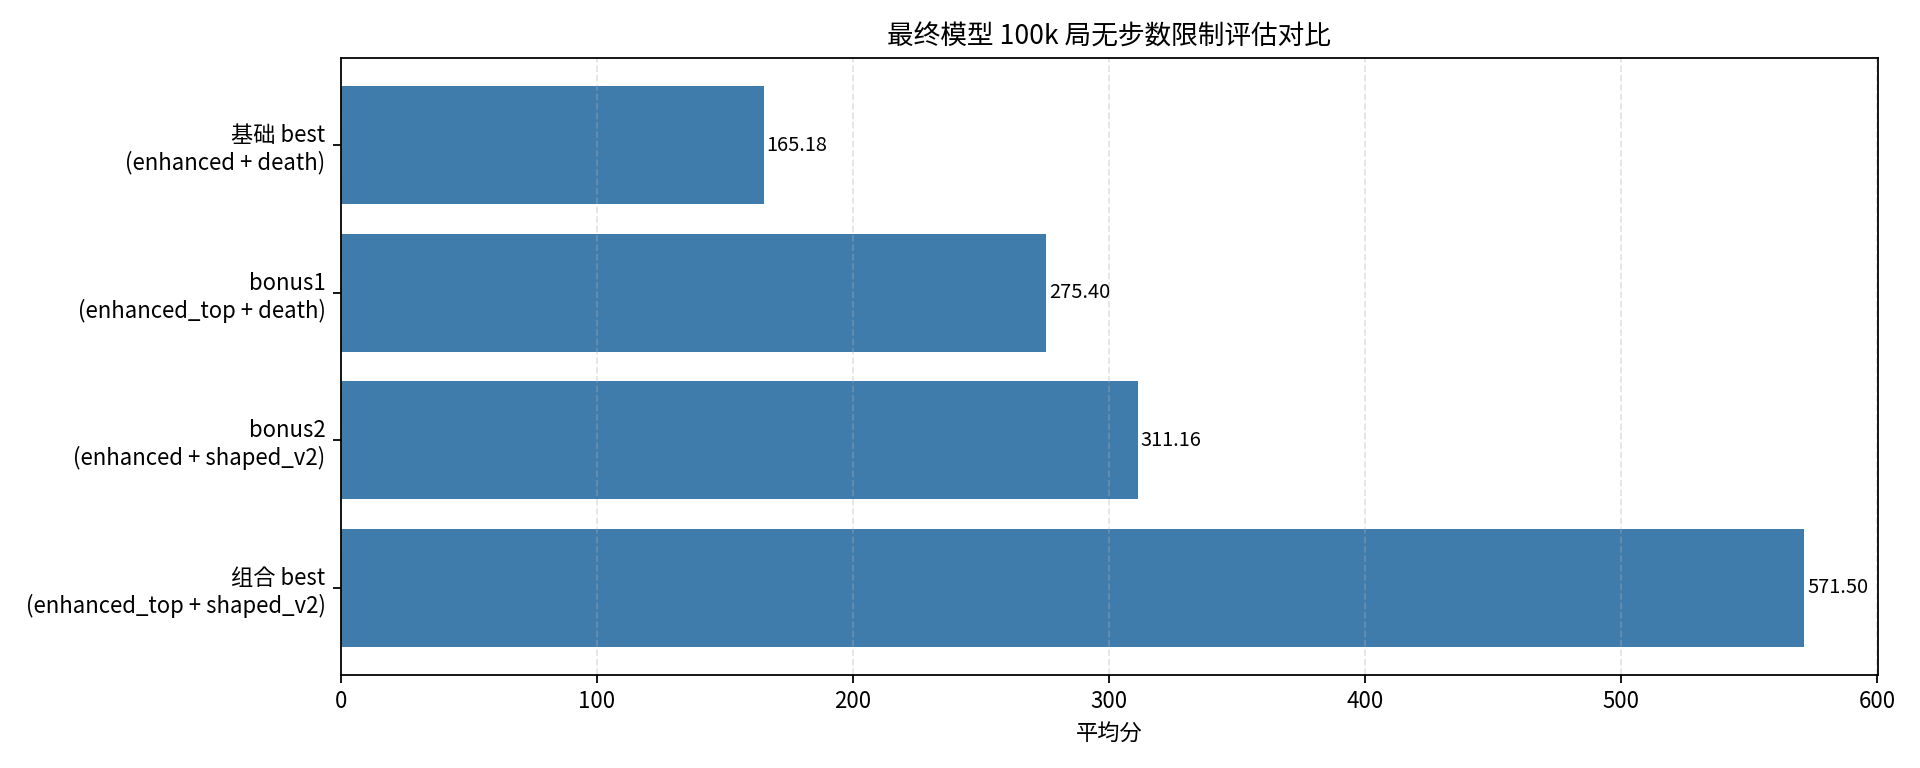
\includegraphics[width=0.85\textwidth]{final_model_compare.png}
	\caption{最终模型 100k 局无步数限制评估对比}
	\label{fig:final_compare}
\end{figure}

如图 \ref{fig:final_compare} 和表 \ref{tab:bonus_final} 所示：

\begin{enumerate}
	\item \textbf{bonus1}（\texttt{enhanced\_top}）：仅增加 $player\_y - pipe\_top$ 一维，均分从 $165.18$ 提升到 $\mathbf{275.40}$（+67\%），Q 表仅增加 $\sim$6k 条目。证明上边界信息是 gaps 导航的关键缺失维度。
	\item \textbf{bonus2}（\texttt{shaped\_v2}）：移除反直觉惩罚、加大中心奖励后均分达到 $\mathbf{311.16}$（+88\%），且方差增大反映模型敢于尝试更激进的穿越策略。
	\item \textbf{组合模型}（\texttt{enhanced\_top + shaped\_v2}）：两项改进叠加产生协同效应，均分达到 $\mathbf{571.50}$，最高分 $\mathbf{2620}$，分别为基础 best 的 $3.5\times$ 和 $2.7\times$。标准差 $615.99$ 说明性能波动较大——模型能跑出极高分会合，但仍在部分种子中过早死亡，与 Q 表对罕见状态的覆盖不足有关。
\end{enumerate}

结论：\texttt{enhanced\_top} 状态和 \texttt{shaped\_v2} 奖励各自独立优于基础方案，两者结合效果更佳。

\section{结论}

本实验使用表格型 Q-Learning 为 Flappy Bird 训练智能体，得到如下结论：

\begin{enumerate}
	\item \textbf{Q-Learning 的有效性}：Q-Learning 能够在离散状态空间中逐步学习状态—动作价值，使智能体在无需了解游戏物理机制的前提下，通过试错获得穿越管道的有效策略。基础最佳模型 50 局无步数限制评估平均 $165.18$ 分，最高 $984$ 分。

	\item \textbf{bonus1 状态改良}：在 \texttt{enhanced}（4 维）基础上增加 $player\_y - pipe\_top$（到上管道距离）形成 \texttt{enhanced\_top}（5 维）。仅增加 1 维使 Q 表规模可控（$\sim$21k），但提供了关键的上边界和间隙大小信息。100k 局训练后均分达到 $\mathbf{275.40}$，比 \texttt{enhanced} 提升 67\%。模型保存为 \texttt{q\_bonus1\_best.pkl}。

	\item \textbf{bonus2 奖励改良}：原版 \texttt{shaped} 的速度惩罚和扇动惩罚与 flap 动作的目标矛盾，中心奖励引导力也不足。\texttt{shaped\_v2} 移除这两个惩罚、将中心奖励放大 5 倍（最大 $+1.0$），100k 局训练后均分达到 $\mathbf{311.16}$（最高 $1271$），比 baseline 提升 88\%，比原版 \texttt{shaped} 提升 185\%。模型保存为 \texttt{q\_bonus\_best.pkl}。

	\item \textbf{组合模型}：将 \texttt{enhanced\_top} 状态与 \texttt{shaped\_v2} 奖励结合，100k 局训练后均分达到 $\mathbf{571.50}$，最高分 $\mathbf{2620}$，为基础 best 模型的 3.5 倍。模型保存为 \texttt{q\_combined\_best.pkl}。

	\item \textbf{最终提交}：基础最佳模型 \texttt{q\_base\_best.pkl}（enhanced + death\_penalty）、bonus1 模型 \texttt{q\_bonus1\_best.pkl}、bonus2 模型 \texttt{q\_bonus\_best.pkl}、组合最佳模型 \texttt{q\_combined\_best.pkl}。
\end{enumerate}

\end{document}
